\subsubsection{HTML}

Mit der steigenden Nachfrage von Webseiten in den 1990er, wurde \gls{html} als strukturierte Möglichkeit vorgestellt, um grafische Webseiten zu erstellen.

Die Basis jeder Webseite ist ein \gls{html}-Gerüst, welches die Struktur und Einzelteile angibt, dabei umfasst der \gls{html}-Standard Überschriften, Paragraphen, Tabellen und Listen. Zusätzlich ermöglicht HTML das Inkludieren von Fotos, Videos als auch von anderen Dokumenten (PDF-Dateien, Webseiten). \cite{HTML-CSS}

Um das Arbeiten mit \gls{html} zu vereinfachen, wurden genau wie bei anderen Technologien für jedes Programm unterschiedliche Plugins eingebunden. Mit der Zeit wurden die Plugins in den Standard eingefasst und damit entwickelten sich über die Jahre unterschiedliche Versionen. Seit Oktober 2014 ist HTML5 als allgemeiner Grundsatz definiert und erhielt seit jeher keine weitere Versionsnummer, da man Änderungen als ''living standard'' weiterentwickelt. \cite{HTML5}

Ein \gls{html}-File (.html, .htm) besteht aus \gls{html}-Tags, welche mit einem kleiner Zeichen ''<'' beginnen und einem größer Zeichen ''>'' enden. Der Inhalt dazwischen unterscheidet sich je nach Komponente (p, h1, a, ...).

Neben dem eigentlichen Tag können HTML-Elemente noch zusätzlich Attribute beinhalten, welche zusätzlich Informationen liefern. Diese werden normalerweise als Name/Value-Paar im Starting Tag aufgelistet. Dabei sind die meisten freiwillig, jedoch gibt es dafür auch Ausnahmen (src-Attribut im img-Tag). \cite{HTML-ATT1, HTML-ATT2}

In der Regel besteht jede Komponente aus zwei \gls{html}-Tags einem Starting Tag und einem Ending Tag, welches noch einen zusätzlichen Schrägstrich ''/'' beinhaltet. Jedoch gibt es Self-Closing Tags als Ausnahme, wo eine Komponente aus einem einzelnen HTML-Tag besteht.

Dieses HTML-File nimmt die Struktur eines Baumes an, das heißt, dass es sich um eine hierarchische Abfolge von Komponenten handelt. Diese Struktur ähnelt der von \gls{xml}, jedoch befolgt es nicht alle Richtlinien von \gls{xml}. Wird diese Kompatibilität vorausgesetzt muss man auf \gls{xhtml} zurückgreifen. \cite{HTML-CSS}

Zu den wichtigsten HTML-Tags gehören: \cite{HTML-Tags}

\begin{table}[H]
    \centering
    \begin{tabular}{|l|p{0.72\linewidth}|}
        \hline
        \lstinline|<h1>| bis \lstinline|<h6>| & Überschrift in unterschiedlicher Reihung (1 = Hauptüberschrift, 2-6 = Unterüberschriften) \\ \hline
        \lstinline|<p>|                            & Paragraph                                                                                 \\ \hline
        \lstinline|<a>|                            & Hyperlink                                                                                 \\ \hline
        \lstinline|<img>|                            & Bild                                                                                      \\ \hline
        \lstinline|<ol/ul>|                            & Geordnete und ungeordnete Liste                                                           \\ \hline
        \lstinline|<li>|                            & Element einer Liste                                                                       \\ \hline
        \lstinline|<strong>|                            & Hebt den Text in Fettschrift hervor                                                       \\ \hline
        \lstinline|<div>|                            & Block-Element                                                                             \\ \hline
        \lstinline|<table>|                           & Tabelle                                                                                   \\ \hline
        \lstinline|<tr>|                           & Tabellenzeile                                                                             \\ \hline
    \end{tabular}
    \caption{Beispiele für HTML-Tags}
\end{table}

Zusätzlich könnten HTML-Elemente diese Attribute enthalten (Auszug):

\begin{table}[H]
    \centering
    \begin{tabular}{|l|p{0.8\linewidth}|}
        \hline
        \lstinline|id| & Mit der Id kann ein HTML-Element direkt referenziert werden                           \\ \hline
        \lstinline|title| & Gibt Zusatzinformationen zu einem HTML-Element, welche als Tooltip dargestellt werden \\ \hline
        \lstinline|disabled| & Gibt an, ob ein HTML-Element benutzbar ist (benötigt keinen Value)                    \\ \hline
    \end{tabular}
    \caption{Beispiele für HTML-Attribute}
\end{table}


Ein gewöhnliches \gls{html}-File beginnt mit \lstinline{<!DOCTYPE html>}, um den Browser mitzuteilen, welcher Datentyp zu erwarten ist. Diese Information unterscheidet sich je nach Version und bei \gls{xhtml}. \cite{DOCTYPE}

Ein \gls{html}-File, welches einen Auszug aus den wichtigsten \gls{html}-Tags beinhaltet, könnte so aussehen:

\lstinputlisting[language=HTML, caption={Beispiel für ein HTML-File}]{code-snippets/index.html}

Wird das vorherige \gls{html}-File in einem gewöhnlichen Browser geöffnet, wird die Struktur folgendermaßen interpretiert:

\begin{figure}[H]
    \centering
    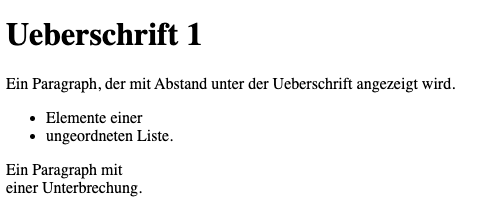
\includegraphics[scale=0.8]{sections/implementation/images/DemoApp.png}
    \caption{Beispiel für ein angezeigtes HTML-File}
\end{figure}